\documentclass[oneside, 11pt]{article}

\usepackage[T1]{fontenc}
\usepackage[utf8]{inputenc}
\usepackage[dutch]{babel}

\usepackage{fouriernc}
\usepackage[detect-all, load-configurations=binary,
            separate-uncertainty=true, per-mode=symbol,
            retain-explicit-plus, range-phrase={ tot }]{siunitx}

\usepackage{setspace}
\setstretch{1.2}

\setlength{\parskip}{\smallskipamount}
\setlength{\parindent}{0pt}

\usepackage{geometry}
\geometry{marginparwidth=0.5cm, verbose, a4paper, tmargin=3cm, bmargin=3cm, lmargin=2cm, rmargin=2cm}

\usepackage{float}

\usepackage[fleqn]{amsmath}
\numberwithin{equation}{section}
\numberwithin{figure}{section}

\usepackage{graphicx}
\graphicspath{{Figures/}}
\usepackage{subfig}

\usepackage{tikz}
\usetikzlibrary{plotmarks}

\usepackage{fancyhdr}
\pagestyle{fancy}
\fancyhf{}
\rhead{\thepage}
\renewcommand{\footrulewidth}{0pt}
\renewcommand{\headrulewidth}{0pt}

\usepackage{relsize}
\usepackage{xspace}
\usepackage{url}

\newcommand{\figref}[1]{Figuur~\ref{#1}}

\newcommand{\hisparc}{\textsmaller{HiSPARC}\xspace}
\newcommand{\kascade}{\textsmaller{KASCADE}\xspace}
\newcommand{\sapphire}{\textsmaller{SAPPHiRE}\xspace}
\newcommand{\jsparc}{\textsmaller{jSparc}\xspace}
\newcommand{\hdf}{\textsmaller{HDF5}\xspace}
\newcommand{\aires}{\textsmaller{AIRES}\xspace}
\newcommand{\csv}{\textsmaller{CSV}\xspace}
\newcommand{\python}{\textsmaller{PYTHON}\xspace}
\newcommand{\corsika}{\textsmaller{CORSIKA}\xspace}
\newcommand{\labview}{\textsmaller{LabVIEW}\xspace}
\newcommand{\daq}{\textsmaller{DAQ}\xspace}
\newcommand{\adc}{\textsmaller{ADC}\xspace}
\newcommand{\adcs}{\textsmaller{ADC}s\xspace}
\newcommand{\Adcs}{A\textsmaller{DC}s\xspace}
\newcommand{\hi}{\textsc{h i}\xspace}
\newcommand{\hii}{\textsc{h ii}\xspace}
\newcommand{\mip}{\textsmaller{MIP}\xspace}
\newcommand{\hisparcii}{\textsmaller{HiSPARC II}\xspace}
\newcommand{\hisparciii}{\textsmaller{HiSPARC III}\xspace}
\newcommand{\pmt}{\textsmaller{PMT}\xspace}
\newcommand{\pmts}{\textsmaller{PMT}s\xspace}

\DeclareSIUnit{\electronvolt}{\ensuremath{\mathrm{e\!\!\:V}}}

\DeclareSIUnit{\unitsigma}{\ensuremath{\sigma}}
\DeclareSIUnit{\mip}{\textsmaller{MIP}}
\DeclareSIUnit{\adc}{\textsmaller{ADC}}

\DeclareSIUnit{\gauss}{G}
\DeclareSIUnit{\parsec}{pc}
\DeclareSIUnit{\year}{yr}



\begin{document}

\title{Dagelijkse controle van een station} \author{C.G.N. van Veen}
\date{}

\maketitle

\section{Stations}

\hisparc heeft verschillende meetstations op scholen in heel Nederland
staan. Aangezien deze stations de hele dag meten en hun data verzenden
naar de \hisparc database, moeten zij regelmatig gecontroleerd worden op
correcte werking. Het station-monitor systeem wat door \hisparc gebruikt wordt heet \emph{Nagios}. 
Informatie over de status van een station is te vinden op \url{http://data.hisparc.nl}. 
Dit document geeft aan hoe te handelen als de status van een station niet optimaal is.

\section{Status van een station controleren}

Als contactpersoon van \hisparc bent u verantwoordelijk voor het
onderhoud van het meetstation op uw school of instelling. Om de
prestaties van het station bij te houden, kunt u eens per dag kijken op
de site: \url{http://data.hisparc.nl}, waarvan in figuur
\ref{fig:frontweb} een screenshot te zien is. Op deze site staan alle
stations, die in het netwerk van \hisparc zijn aangesloten, vermeldt. De
cirkels voor de stations geven met een kleurcode aan wat de status van
een station is. Als de kleur van de cirkel voor het betreffende station
groen is, dan is de status van het station 'in orde'. Een gele cirkel
geeft aan dat er een probleem is met het station. Een rode cirkel
betekent dat er geen data van het station ontvangen wordt en dat het
station dus niet werkt.

\begin{figure} \centering 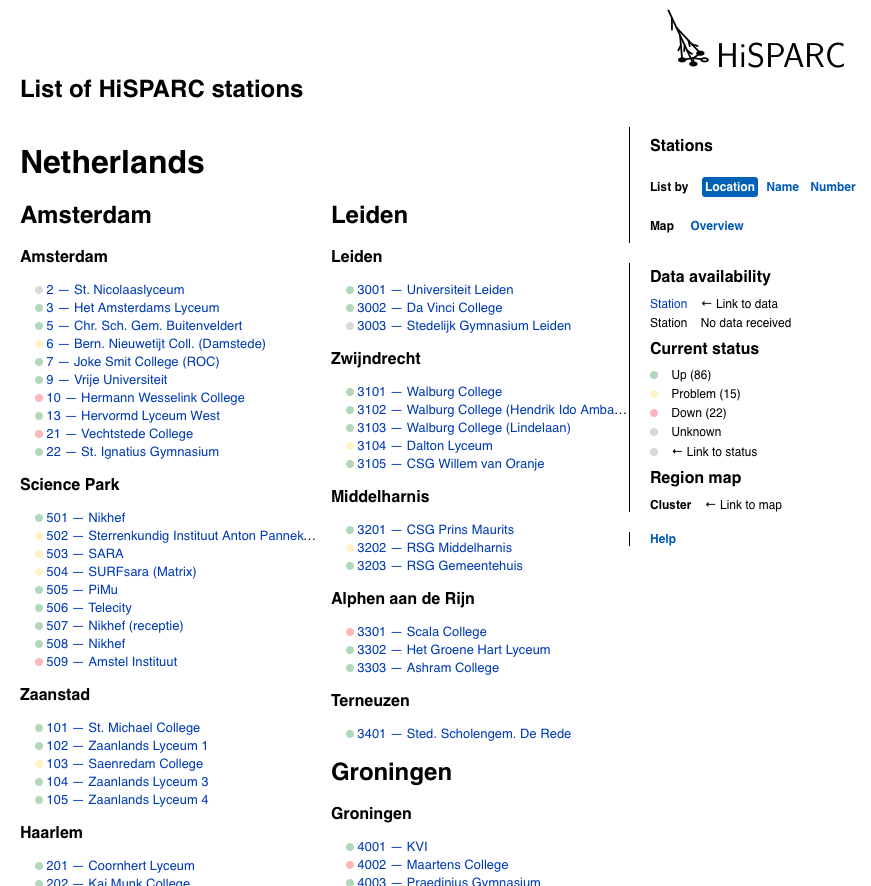
\includegraphics[scale=0.60]{websitefront}
\caption{Vooraanzicht van de \hisparc website.} \label{fig:frontweb}
\end{figure}

\section{Probleem met een station}

In het geval van een gele of rode cirkel, kunt u klikken op de link van het
desbetreffende station (bijvoorbeeld klikken op: \underline{501-Nikhef}) zoals te zien is in figuur \ref{fig:frontweb}. 
Dan wordt u doorgelinkt naar de status pagina van het betreffende station. Zo'n
pagina met een overzicht van verzonden data van een station is weergeven
in figuur \ref{fig:websiteproblem}. In figuur \ref{fig:websiteproblem}
is te zien dat het station niet meer meet na 14.00 uur,  omdat het aantal
gemeten events naar nul gaat. In het Pulseheight histogram is ook te zien
dat \mip piek niet goed aanwezig is, wat duidt op een verkeerde
instelling van de \pmt. Zie ook \cite{inregelen} elders in dit boekje.

\begin{figure} 
\centering 
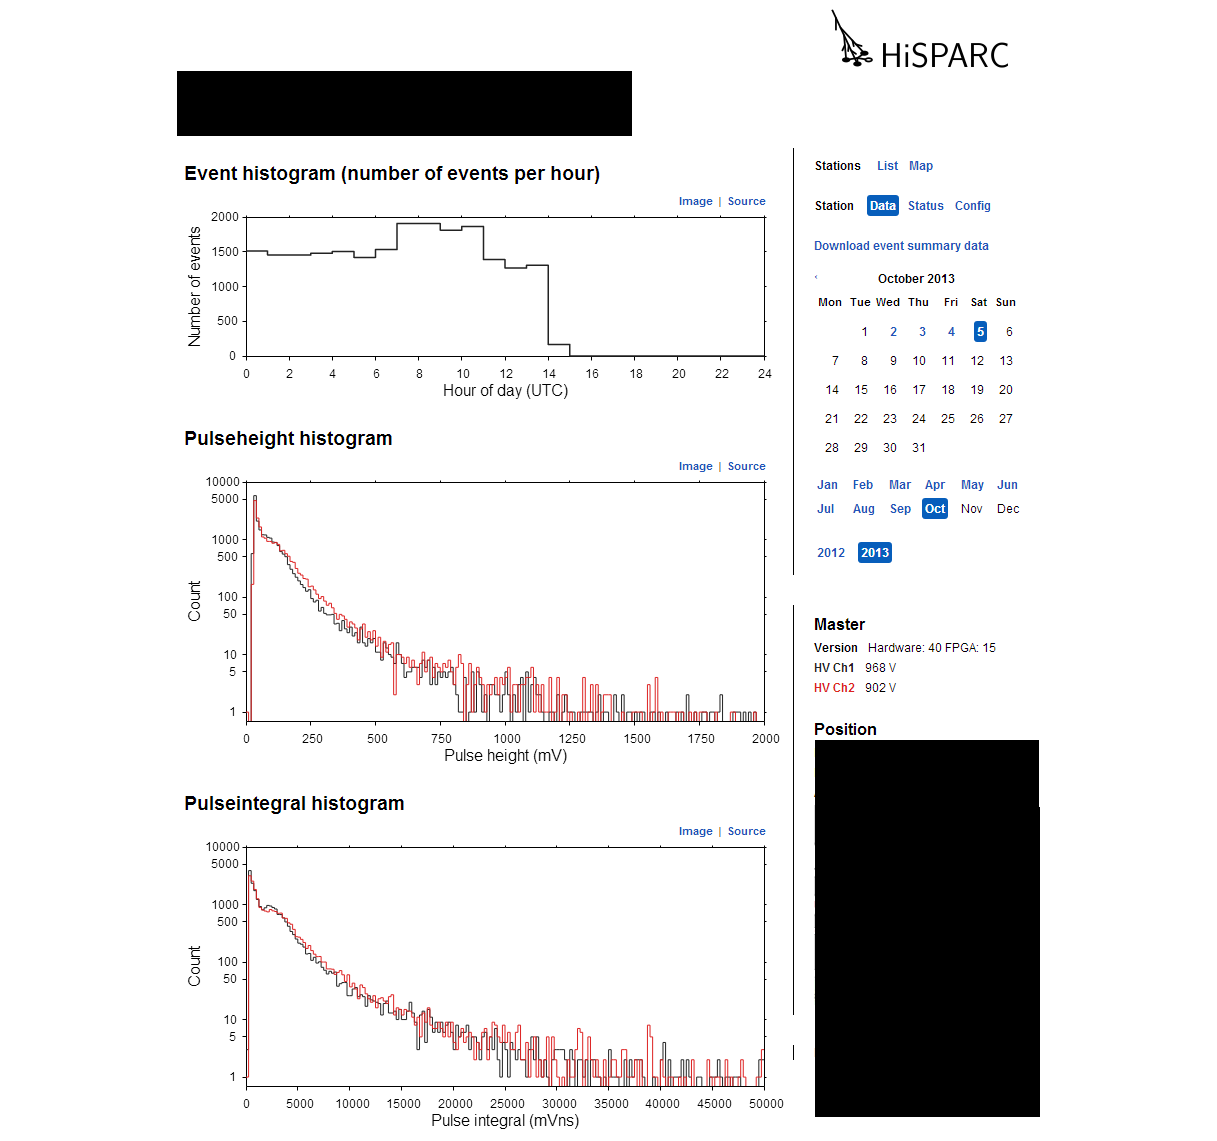
\includegraphics[scale=0.40]{websiteerror}
\label{fig:websiteproblem} 
\caption{Screenshot van het data-overzicht van een
station. In het event histogram is duidelijk te zien dat het station
niets meer meet na 14.00 uur. Ook is er in het Pulseheight histogram
geen duidelijke MIP piek te zien.} 
\end{figure}

\section{Problemen oplossen}

Om precies te zien wat er mis is met het station en het probleem
daadwerkelijk op te lossen, klikt u op het cirkeltje voor het station.
Dan krijgt u een status en problemen overzicht. In figuur \ref{status_station} is te zien dat de \verb|TriggerRate|
rood is en dus aandacht behoeft.
Om de problemen met de verschillende categorieën op te lossen is een speciale website ontwikkeld.
Ga naar \url{http://http://docs.hisparc.nl/maintenance/}. Klik hier op \emph{frequently asked questions} en daarna op \emph{known issues}. Op de site "known issues"  kun je een gecategoriseerde lijst van problemen zien. Je kunt op probleem zoeken en dus in ons geval in de derde regel klikken op \emph{TriggerRate}. Op de site verschijnt dan een lijst met problemen die een foutmelding "TriggerRate" geven. 
Door nu in deze lijst te kijken, is een oplossing te vinden voor de instelling.
In ons voorbeeld kijken we bijvoorbeeld naar een foutmelding op de TriggerRate en vinden dan als mogelijke reden:
De button "DAQ Mode" is niet aangevinkt, met oplossing om deze aan te vinken.

Bij andere problemen met stations kunt u het bovenstaande stappenplan op dezelfde manier volgen om diverse storingen en problemen met u station op te lossen.
Komt u er alsnog niet uit neem dan contact op met:........................
 

\begin{figure} 
\centering 
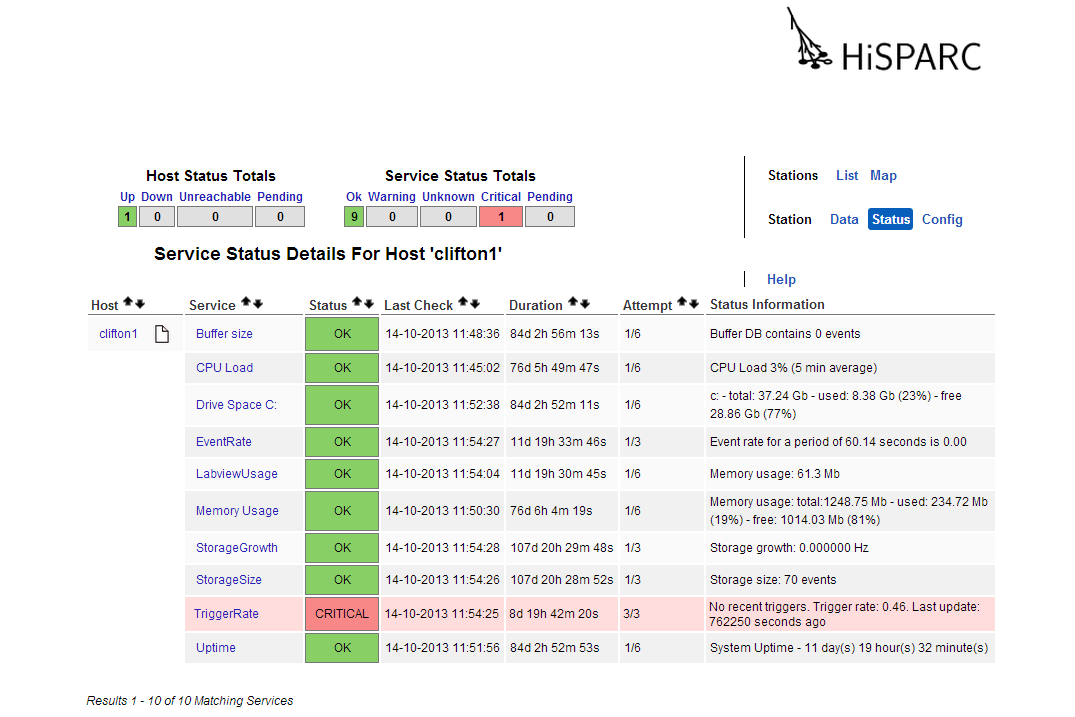
\includegraphics[scale=0.60]{status_station}
\label{fig:status_station} 
\caption{Screenshot van de status van een
station. In de tabel is in rood aangegeven welke foutmeldingen er voor het station zijn waargenomen. In dit geval is er een probleem met de TriggerRate.} 
\end{figure}

\begin{figure} 
\centering 
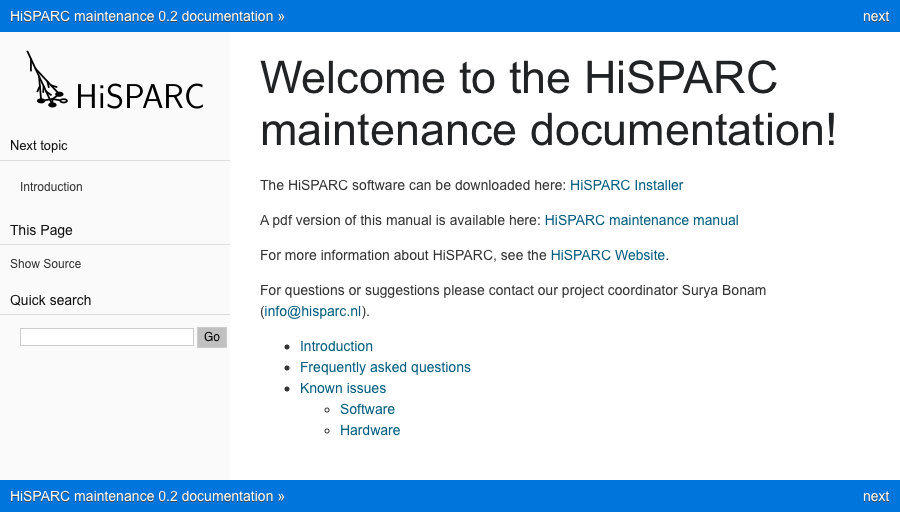
\includegraphics[scale=0.60]{maintenance}
\label{fig:maintenance} 
\caption{Klik op \emph{frequently asked questions} en daarna op \emph{known issues} om naar verschillende foutmeldingen en oplossingen daarvan te gaan.} 
\end{figure}
 
\begin{figure} 
\centering 
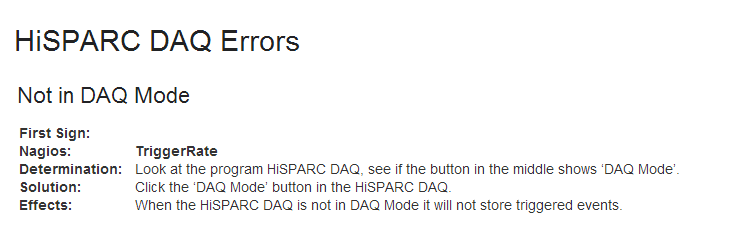
\includegraphics[scale=0.60]{solution}
\label{fig:solution} 
\caption{Een mogelijke reden voor foutmelding en de bijhorende oplossing. Op \emph{http://http://docs.hisparc.nl/maintenance/known-issues.html} Hier is de oplossing, om in het programma \hisparc DAQ de button "DAQ mode" aan te vinken.} 
\end{figure}




\begin{thebibliography}{9} 
	
	\bibitem{inregelen} D.B.R.A. Fokkema, \emph{Inregelen PMT's}, infopakket \hisparc 
\end{thebibliography}



\end{document}
